\documentclass[conference]{IEEEtran}

\usepackage{hyperref}
\usepackage{graphicx}\graphicspath{ {images/} }
\usepackage{listings}
\usepackage{flushend}

% Hyphenation correction
\hyphenation{op-tical net-works semi-conduc-tor}


\begin{document}

\title{A Lightweight Encrypted Access Control System}
\author{\IEEEauthorblockN{Stuart Miller}
\IEEEauthorblockA{Department of Electrical and\\Computer Engineering\\
Missouri University of Science \& Technology\\
Rolla, Missouri 65409\\
Email: sm67c@mst.edu\\
Web: \url{http://web.mst.edu/\textasciitilde sm67c}}
}

\maketitle

\begin{flushright}\end{flushright}
\begin{abstract}
The Data Encryption Standard (DES) block cypher algorithm is a vital piece of computing history. Although DES is no longer considered to be secure, an analysis of the need for and means of implementing DES proves to be an insightful lesson in the need for it's successors. In particular, this paper will focus on the implementation of DES on an 8051 microcontroller, an 8-bit platform that was common when the algorithm was designed. DES proves highly applicable to 8-bit programming methodologies and is easily computed on such a low-power platform. Throughout the following design of an access-control system, protected with DES encryption, such benefits will be enumerated.
\end{abstract}

\section{Introduction}
The use of encryption is so exceedingly commonplace in today's technology that it is often taken for granted. The fact that one's banking transactions are secure today is simply an unstated expectation. Encryption is everywhere; even in the seemingly transparent viewing of webpages, encryption is working behind the scenes to ensure that data cannot be stolen by malicious actors. However, technology has not always had such security so deeply ingrained. To better understand the need for and design of encryption today, it is necessary to examine the history of encryption. The design of the first encryption algorithm was truly the catalyst that allow the modern internet to grow to what it is today.

Historically, the time of the late 1960s and early 1970s saw an immense amount of technological change in the field of computing. A survey of the field at the time identified several areas that were increasingly heavily reliant on computer power: communications, electronic surveillance, management of time-sensitive data, even the day-to-day business of geographically distanced corporations or governments\cite{des_survey}. Threats could come from attempts to gain market information in the private sector, attempts to gain market information from government agencies, intentional fraud through banking, law enforcement, or economic data, and invasion of personal private information. This new-found prevalence made the threat of information theft highly appealing at the time. As such, the need for digital encryption was pressing, both for governments and the private sector.	

The Data Encryption Standard (DES) was introduced in 1976 as FIPS standard 46 (it exists today as FIPS revised standard 46.3\cite{fips_46_3}). DES solved the problem of information theft by introducing an industry-wide standard for secure encryption. This introduction catalyzed the field of modern computational cryptography and remain relevant for many years after its introduction.

In order to examine the significance and relative prosperity of the DES algorithm, an analytical approach will be taken to implementing the DES algorithm on an 8051 microcontroller. The hardware used will be a Phillips (NXP Semiconductor) P89LPC932A1FA \cite{8051_datasheet}. This is an 8-bit 8051 architecture, clocked at 12MHz, with 256 bytes of data memory, 512 bytes of auxiliary memory, and 8kB of code flash memory.

\section{About DES}
The introduction of DES has its roots during World War II code-breaking efforts. American cryptographer Claude Shannon was among the first to describe the system of private key encryption in 1945. Figure \ref{fig:shannon_private_key} shows Shannon's depiction of a private key encryption scheme, same as the one used by the DES algorithm. 
\begin{figure}[ht]
	\centering
  \includegraphics[width=3.4in]{shannon_private_key.png}
  \caption{Shannone's private key encryption scheme\cite{shannon}}
  \label{fig:shannon_private_key}
\end{figure}
In addition to describing the methodology for private key encryption, Shannon is also credited with proposing the concepts of confusion and diffusion; novelties which DES was the first to make effective use of\cite{shannon}. The concepts are descried as follows:
\begin{itemize}
  \item Confusion - the  relationship between an element of the plaintext and the ciphertext should be complex and involve several parts of the key
  \item Diffusion - changing a single element of the plaintext should change multiple elements of the ciphertext
\end{itemize}
DES makes use of a Feistal cipher design, meaning plaintext is encrypted iteratively in rounds. Since each round involves lateral bit-shifts and bit-by-bit addition modulo 2, (the XOR operation) both diffusion and confusion are achieved.

Throughout the late 1990s and even into the early 2000s, 8-bit architectures were enjoying a prosperous presence. Williams states in his 1999 journal article that 8-bit architecture are "rapidly becoming universal" and are "economically very rewarding" \cite{8_bit_alive}. Even though the 8051 architecture dates from the 1970s, the platform showed great success well into the next century and undoubtedly had a large part in the rise and persistence of the DES algorithm. This is because DES operates on a 64-bit block size, with a 56-bit key. (Note that for simplicity's sake,m keys are sometimes rounded up to 64 bits just to have a nice round size, but the algorithm will discard the last 8 bits.) This makes it easy to break up interative operations into 8-bit sizes. Furthermore, the mathematical operations involves are simple, consisting only of shift and XOR operations, both of which are native to 8-bit hardware.


\section{Program Structure}
The actual code required to implement DES is surprisingly simply. When all the structural overhead and comments are removed, the significant code is less than 100 lines. This speaks greatly to the simplicity of the algorithm's design. Conversely, the overhead comes in the maintenance of a large number of static variables. The DES algorithm requires eight substitution boxes (S-boxes) and several permutation matrices. The inclusion of all these actually requires more data memory than the device possesses. Fortunately, this chip includes additional xdata, where the variables can be stored. The code compilation listing report (Figure \ref{fig:compilation_report}) shows 1134 bytes of XDATA memory were utilized.
\begin{figure}[ht]
	\centering
  \includegraphics[width=2.75in]{compilation_report.png}
  \caption{Keil C51 Code Listing Report}
  \label{fig:compilation_report}
\end{figure}
\begin{figure}[ht]
	\centering
  \includegraphics[width=3.2in]{des_algorithm.png}
  \caption{DES Algorithm Flow \cite{fips_46_3}}
  \label{fig:des_algorithm}
\end{figure}

\subsection{Algorithm Portability}
At the highest level, the DES encryption algorithm involves just a simple call to \texttt{\textit{des\textunderscore encrypt(key, message)}} or \texttt{\textit{des\textunderscore decrypt(key, message)}}. This encapsulates the algorithm quite nicely and can be reused across multiple projects easily. The fact that DES requires no advanced setup or configuration whatsoever speaks to the portability of the algorithm and is undoubtedly indicative of its popularity.

\subsection{Structure}
As shown in Figure \ref{fig:psuedo}, the actual process of DES is quite simple and easy to implement. The convenient part of the DES structure is that it makes use of a lot of reusable components. Permute operations happen quite frequently; the SBoxes rely on permutations as to the initial(IP) and final(FP) permutations and permuted choice 1(PC1) and 2(PC2). Also used often are shift, split, and combine operations. These can all be written as simple reusable functions and implemented as needed throughout the algorithm for the sake of clarity.

Each of the permutation tables (IP, FP, PC1, PC2, and all 16 S-Boxes) are written into the 8051's code memory. There is absolutely no need to keep these in data memory as they remain static and take up quite a bit of space.

\begin{figure}[ht]
  \centering
  \begin{lstlisting}[language=C,frame=single,tabsize=3,breaklines=true,basicstyle=\small]
	// Generate keys (x16)
	permute(key, PC1);
	split(key, keyLeft, keyRight);
	for 0->16
		shift(keyLeft);
		shift(keyRight);
		key = combine(keyLeft, keyRight);
		if(type == ENCRYPT)
			keys[i] = permute(key, PC2);
		else // type == DECRYPT
			keys[15 - i] = permute(key, PC2);
	}
	
	// Run encryptions rounds (x16)
	permute(plainText, IP);
	split(plainText, left, right);
	for 0->16
		left = right;
		right = permute(right, E) XOR keys[i];
		sBoxTransform(right);
		permute(right, P);
	}
	
	combined = combine(right, left);
	ciphertext = permute(combined, FP);
  \end{lstlisting}
  \caption{DES core function psuedocode}
  \label{fig:psuedo}
\end{figure}


\subsection{8-Bit Affinity}
The 8051 processor makes use of an 8-bit complex instruction set (CISC) architecture. This may, at first, seem like a disadvantage when faced with DES's large 64-bit input size; conversely, it becomes an advantage. Every single sub-block size mandated by the DES algorithm is a multiple of 8. Most of the work occurrs when the 64-bit input is divided into 32-bit halves.

DES also makes extensive use of single bit manipulation as part of the S-Boxes. In this case, each bit substitution must be a distinct action, meaning higher order processors achieve no benefit from having large widths. In this case, the low-cost, low-power 8051 architecture 

Furthermore, DES makes use exclusively of XOR and shift operators, both of which are native to the 8051 instruction set.

\subsection{Converse: Challenges of 8-Bit}
While DES does segment nicely into 8-bit segments, the fact that it does segment at all does provide some detriment to the implementation. For example, where shifting is required, to shift a 32-bit half, the algorithm must shift 7 bits over and carry the 8th bit over to the beginning of next 7 bits. This carry-over requires additional steps and when repeated 4 times over the 32 bits each time, does contribute a significant amount to the required runtime. 

Such repetition over 8-bit boundaries occurs a few more times over the course of the algorithm. In general, every time a value must be operated on, that operation must occur four or eight times, to cover the length of the array.

While such considerations are indeed a disadvantage to implementation on this platform, they are far outweighed by the benefits of being cost-effective, low-power, and simple to operate.

\section{Test Results}
\subsection{Validation}
Examples of encryption and decryption. Verification of algorithm can be seen in Figure \ref{fig:example}. Encoding the plaintext with the 56-bit key yields the ciphertext.

This particular encryption had to be done in two round since the input was greater than 64 bits. Also notice that since the block of plaintext was slightly less than 64 bits, it had to be padded with zeroes. This is a perfectly acceptable strategy, as the property of diffusion ensures that the encryption is still secure even with a large zero-pad at the end. For as long as the attacker does not have prior knowledge of the plain text (i.e. they are looking at just the ciphertext alone, this is just as secure as padding with random values.

\begin{figure}[ht]
  \centering
\begin{tabular}{ | l || l | p{1.4in} | }
  \hline
  & ASCII & Hexadecimal\\
  \hline\hline
  Key & testtest & 74 65 73 74 74 65 73 74 \\
  Plaintext & Hello world! & 48 65 6c 6c 6f 20 77 6f 72 6c 64 21 00 00 00 00 \\
  %ÛX+*ݬɨôPà`\tÓ
  Ciphertext & [unprintable] & 22 db 58 2b 2a dd 19 ac c9 a8 f4 50 e0 60 09 d3 \\
  \hline
\end{tabular}
  \caption{Encryption validation}
  \label{fig:example}
\end{figure}

\subsection{Timing Analysis}

While a working algorithm is important, it is of no value if the algorithm cannot complete within a reasonable runtime for human use. For a single block of DES encryption, this should be indistinguishable to a human. Figure \ref{fig:timing} shows the discrete cycle count for each individual operation, accounting for the 11.0592MHz clock on the 89LPC932A1. Both operations fall in the neighborhood of 50ms, which is a good enough time.

The reason for the difference between the times is due to the implementation of the encrypt/decrypt algorithm. While it is indeed the same algorithm to encrypt and decrypt, decrypt requires generating the keys in reverse order, hence the need take the additional step of calculate from the end of key array rather than the beginning (Figure \ref{fig:diff}). 

Taking this time scale, the time to encrypt various bodies of text is shown in Figure  \ref{fig:timing_table}. The timing table also show the runtime on a modern desktop computer. To achieve the last column, the algorithm was ported to the GNU C compiler and ran on a 64-bit Linux system. Note that that algorithm was not optimized to use 64-bit data types; rather used as-is to provide a comparison for runtime on a standard modern computer system. The resulting runtimes are, of course, much faster. It is rather impractical to consider the runtime to encrypt texts as long as a book; this platform was not designed for such purposes. The target application of DES on an 8-bit system is merely encryption of a short password, PIN code, or perhaps a short message such as a text or tweet. All of these can be encrypted on the 8051 platform within a reasonable runtime.

\begin{figure*}[ht]
  \centering
\begin{tabular}{ | l r r r | }
  \hline
  Body of Text & Characters & Encryption Time (8051) & Encryption Time (GNU C) \\ 
  \hline\hline
  4-digit PIN & 4 & 52.17 ms & 15.04 $\mu$s \\
  "Hello world!" & 12 & 104 ms & 30.80 $\mu$s \\  
  Tweet & 140 & 0.91 sec & 0.270 ms \\
  Gettysburg Address & 1,479 & 9.65 sec & 3.51 ms \\
  US Constitution & 32,026 & \** 3.48 hours & 127.34 ms\\
  Holy Bible  & 3,566,480 & \** 6.46 hours & \** 11.32 s \\
  Entire Harry Potter Series  & 4,878,765 & \** 8.84 hours & \** 15.49 s \\
  \hline
\end{tabular}
  \caption{Timing Analysis (\**timing data for starred entries extrapolated and not measured experimentally) }
  \label{fig:timing_table}
\end{figure*}

\begin{figure}[ht]
  \centering
\begin{tabular}{ | l r r | }
  \hline
  Operation & Instructions & Time \\ 
  \hline\hline
  Encrypt & 576,962 & 52.17ms \\  
  Decrypt & 573,426 & 51.85ms \\    
  \hline
\end{tabular}
  \caption{DES Timing Analysis}
  \label{fig:timing}
\end{figure}

\begin{figure}[ht]
  \centering
  \lstinputlisting[language=C,breaklines=true,firstline=209,lastline=212,tabsize=3,frame=single,basicstyle=\small]{../des.c}
  \caption{Single difference between encryption and decryption}
  \label{fig:diff}
\end{figure}

\section{Expansion Into 3DES}
Unfortunately, DES was not to last. DES was cracked in 1998 by the Electronic Frontier Foundation (EFF) using purpose built hardware to perform a brute-force search \cite{des_cracker}. DES uses a keylength of 56-bits, meaning that there are 2\textsuperscript{56} (or about 72 quadrillion) possible keys. This seemed enough to be computationally secure in the 1970s, when DES was proposed, but by the late 1990s, this figure was rapidly becoming approachable. In 1998, the EFF's \$20 million machine cracked DES in just 56 hours \cite{des_cracker}. DES was subsequently rendered no longer secure.

To remedy this, the triple DES (3DES) algorithm was proposed. 3DES simply runs DES three times in a row, tripling the size of the key. Figure \ref{fig:3des_flowchart} shows the basic methodology. Encryption is achieved by encrypting the plaintext with the first 56 bits of the key, decrypting that result with the next 56 bits of the key, and finally encryption that result with the last 56 bits of the key. Decryption is the opposite process.

As such, it is quite easy to expand an existing DES implementation into 3DES. Figure \ref{fig:3des_diff} shows how this was achieved in just a few lines of code. Figure \ref{fig:3des_timing} shows a timing analysis of 3DES implemented on the 89LPC932A1 microcontroller. As to be expected, it takes rought three times the runtime of DES.

Even so, 3DES has fallen out of common use, replaced by the more recently developed advanced encryption standard (AES), while not entirely obsolete, most application make use of AES instead due to its variable length key size, faster runtime, and higher degree of computational security.

\begin{figure}[ht]
	\centering
  \includegraphics[width=3.4in]{3des.png}
  \caption{Triple DES (3DES algorithm flow}
  \label{fig:3des_flowchart}
\end{figure}

\begin{figure}[ht]
  \centering
  \lstinputlisting[language=C,breaklines=true,firstline=444,lastline=457,tabsize=3,frame=single,basicstyle=\small]{../des.c}
  \caption{3DES functional implementation}
  \label{fig:3des_diff}
\end{figure}

\begin{figure}[ht]
  \centering
\begin{tabular}{ | l r r | }
  \hline
  Operation & Instructions & Time \\ 
  \hline\hline
  Encrypt & 1713292 & 154.92ms \\  
  Decrypt & 1713408 & 154.93ms \\    
  \hline
\end{tabular}
  \caption{3DES Timing Analysis}
  \label{fig:3des_timing}
\end{figure}

\section{Physical Security}
While the effort put into computation security is not without purpose, it is meaningless unless complemented with adequate physical security. For example, say an encryption system such as this was to be connected to a numeric keypad for opening a parking lot gate. The keypad is wired to a computer in a nearby control room, which then encrypts the code that was entered, sends it over the internet to a central database, which then decrypts it and checks it against the valid code for that gate. This systems successfully deters any malicious actors on the internet from determining the access code. It fails to address the issue of physical security. Since the numeric entry keypad must ba accessible outide the gate, the code is traveling to the parking lot control room unencrypted first. An attacker could easily unearth the wiring for the control panel easily install a simple monitoring device which record encrypted passwords, thereby rendering all the network security useless. The solution for this is simple, to encapsulate all components that deal with unencrypted data. The numeric keypad must include the microprocessor and be able to compute the encrypted data right at the keypad. This was, the entire unit can be printed on a single circuit board and build securely into a single tamper-proof enclosure. The circuit board is shown in Figure \ref{fig:board_pic}. One can easily image a rectangular metal housing to seal and protect the circuitry from attackers.

Additionally, to protect against ciphertext reuse, the plaintext or key could be padded with a nonce for additional obscurity. For example, the time of day could be used, or an algorithmically generated sequence, or even something as simple as a counter that increments at every encryption attempt. Any of these would be sufficient to change the ciphertext at every entry, while still remaining computationally secure to attackers, and easily decipherable to the indented receiver.

Combining this physical security with an adequate pattern of to protect against ciphertext reuse can create a highly secure system.

\subsection{Peripherals}
In order to maintain physical security, the microcontroller can be made to comply with a number of standards. Universal asynchronous receiver/transmitter (UART) communication over a serial cable is common, as is pictured in Figure \ref{fig:board_pic}. This board comes with push buttons soldered directly onto the circuit board with direct connection to the P1 and P2 buses of the microcontroller. This solution is preferable to maintain physical security. It may also be desired to implement an LCD module to display the plaintext entered by the user. In a similar manner, a direct connection to the circuitboard would be preferred.

For the purposes of this report, all validation has been done over UART communication with a desktop computer. Input and output values were entered in such a manner. The main reason for this was the lack of a tenth input button on the included circuitboard, disallowing full numeric input, and making alphabetic input more challenging. UART serves an an acceptable means of communication for the purposes of analysis here. Additionally, the Keil C51 development package contains a highly accurate 8051 debugger which emulates actual hardware within the development. Cycle counts and and initial validation were obtained through this emulator.

\begin{figure}[ht]
	\centering
  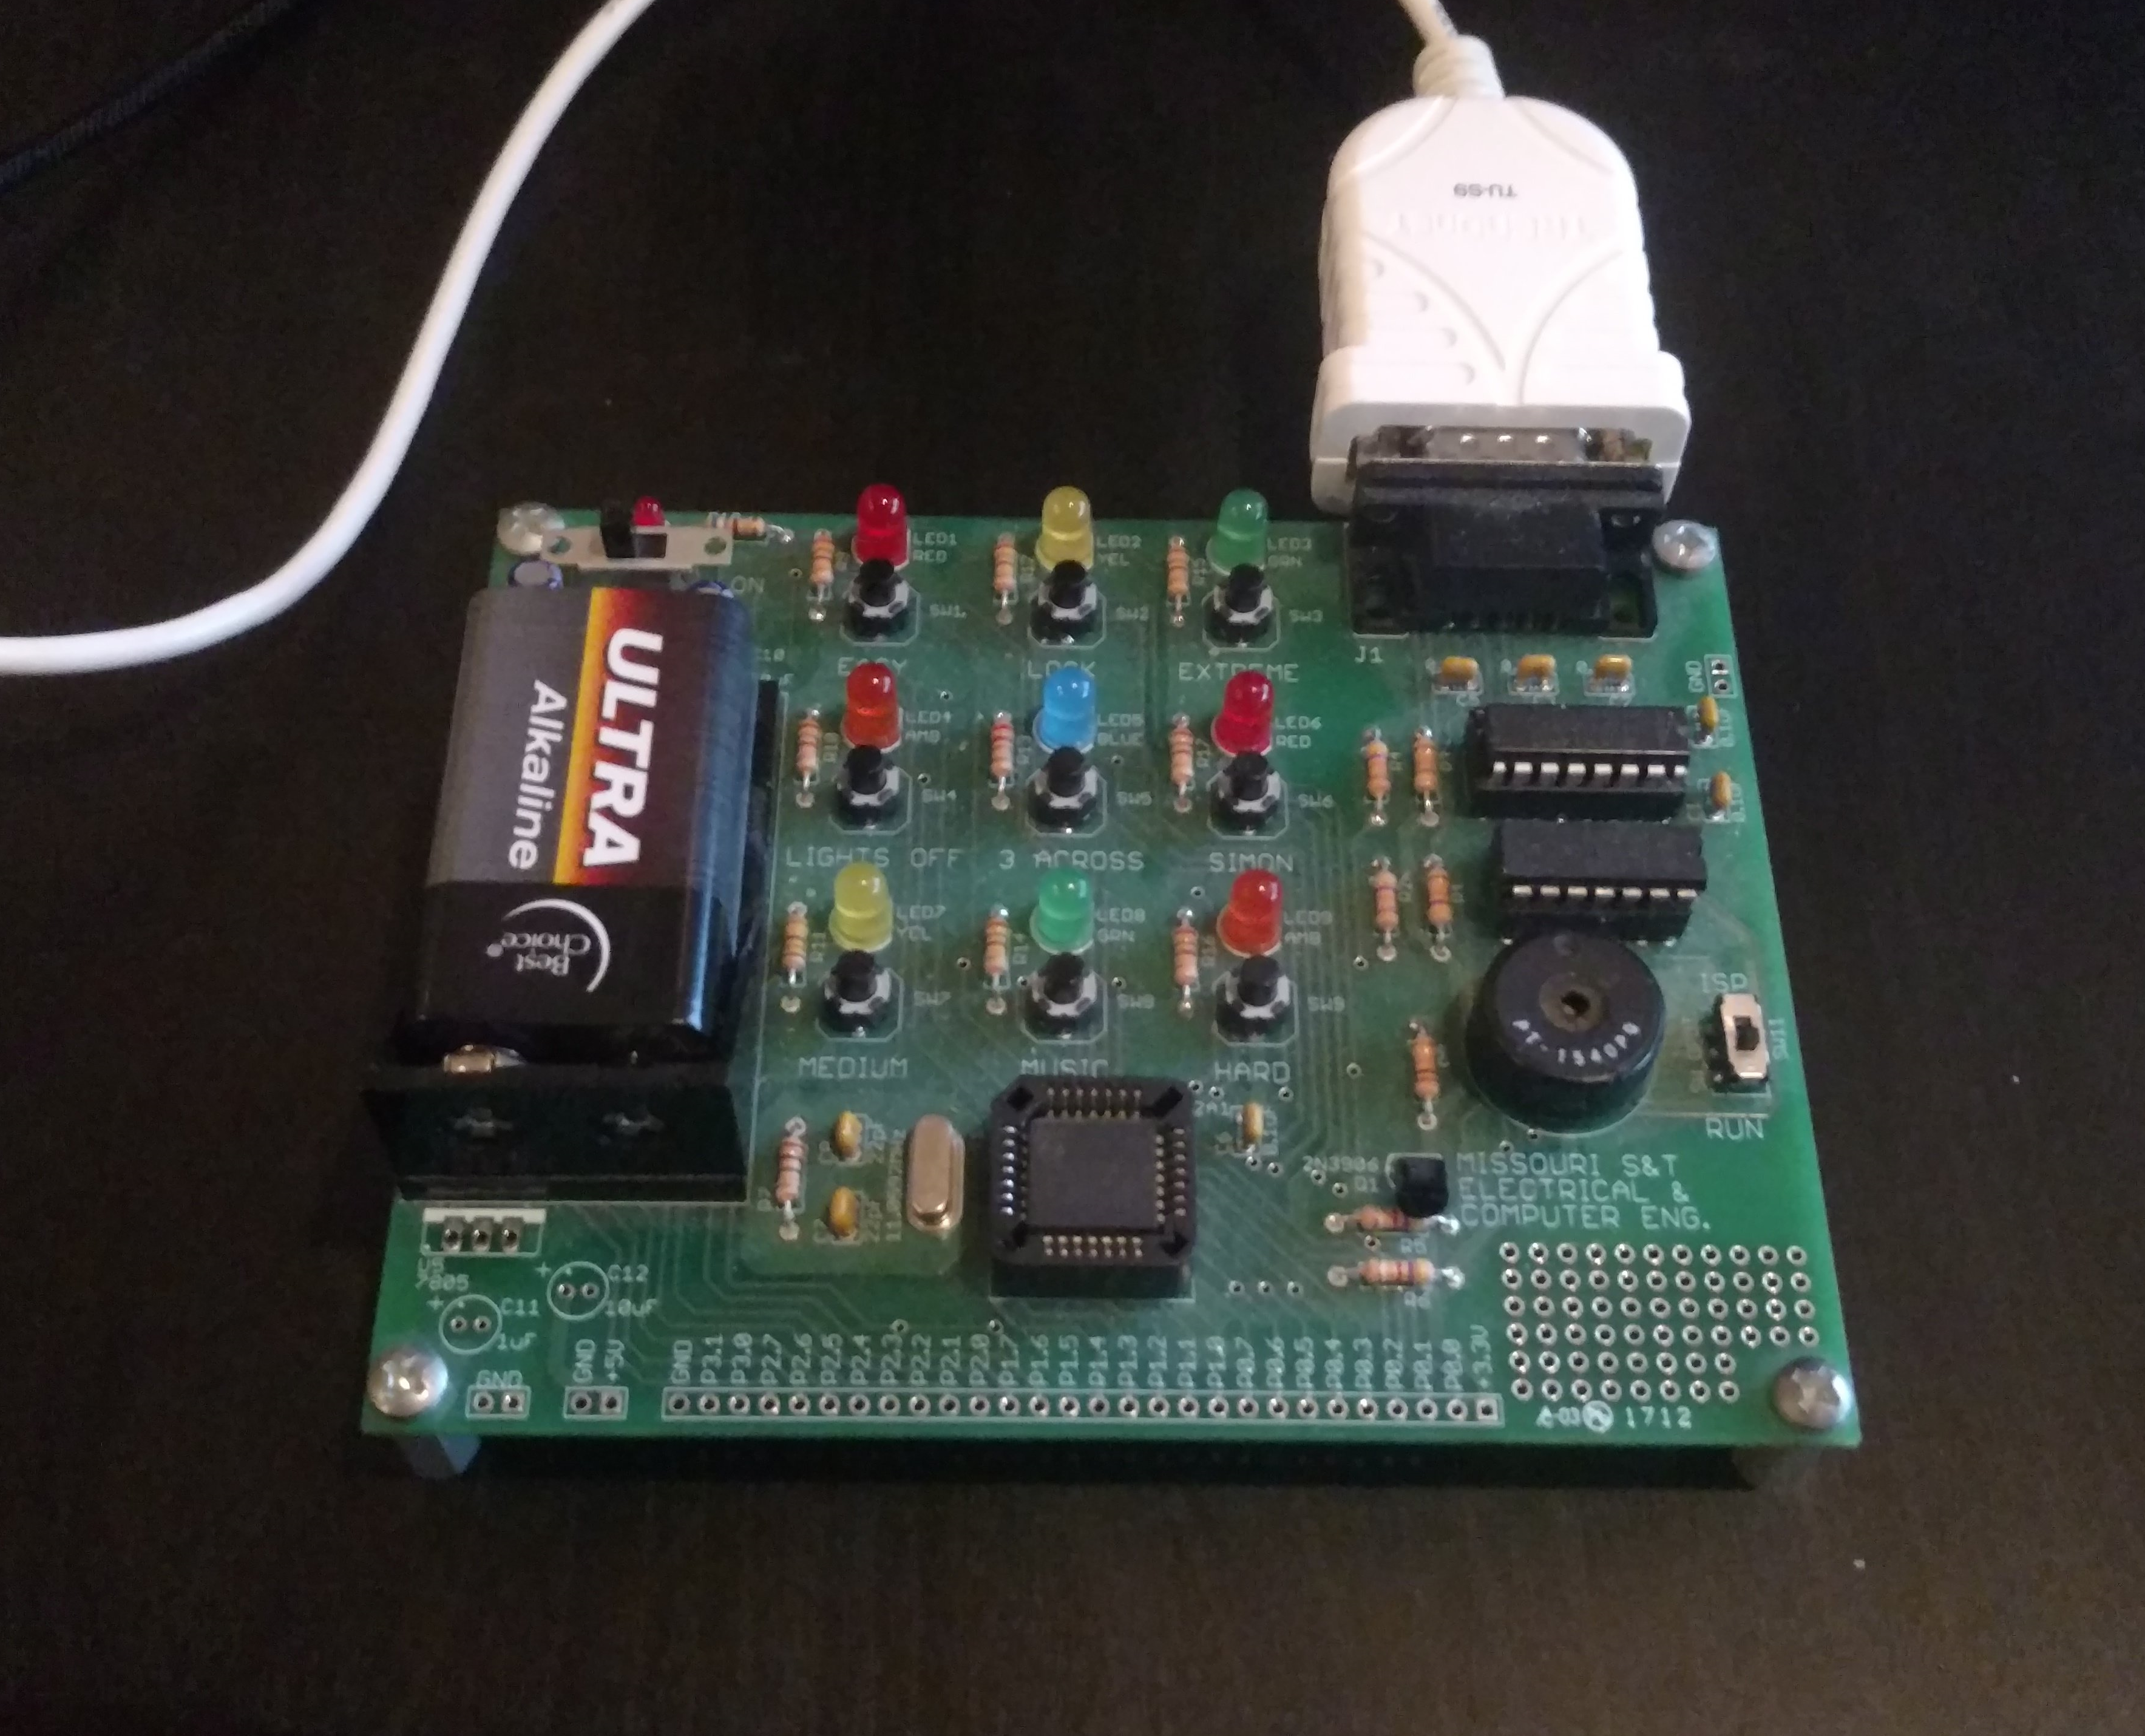
\includegraphics[width=3.2in]{board_pic.png}
  \caption{Missouri S\&T ECE Dept. Simon2 Development Board containing an 89LPC932A1 8051-series microprocessor}
  \label{fig:board_pic}
\end{figure}

\section{Conclusion}
The 8051 architecture, and the 8-bit architecture in general, provides a valuable and cost-effective platform for implementing the DES algorithm. While the algorithm is now obsolete, the lessons learned about implementation on the 8051 platform remain vital to the field of cryptography today. In order to maintain security, physically secure devices are required to maintain encryption at all points along the chain of communication. Today, this involves newer platforms that are more powerful than the 8051, but the desire to remain on the low-power, small form factor side of the market remains.

Another valuable point is the ease of implementation. One of the core requirements of cryptography is that it must be computationally secure, while still remaining accessible to indented user(s). The codebase required to implement DES is remarkably straightforward and thus, it is easy to port the code into an already existing infrastructure.

Overall, DES remains a valuable tool and has provided the foundation for developing modern cryptographic algorithms. The principles of confusion and diffusion, first shown in DES, remain vital to this day. Even the process of breaking the DES algorithm remains a valuable lesson that cryptanalysts should always be striving to push the boundaries of present technology. 

\bibliographystyle{IEEEtran}
\bibliography{sources}

\end{document}



